\section{Proposed Measurement}\label{sec:measurement}
This section is a description on how the \etaDal \ was simulated and reconstructed for this CLAS12 proposal.
\subsection{Simulation and Reconstruction}
To simulate the reaction in Eq.~\ref{eq:etaP}, the program PLUTO++~\cite{PLUTO} was utilized for its ability to simulate the decays of those according to QED, Vector Meson Dominance or a user defined TFF. For reconstruction of the desired topologies, the CLAS12 parameterized Monte-Carlo, FASTMC~\cite{fastmc} was used, in which $\sim 5\cdot10^8$ events were generated for \etaPDal \ and then simulated with FASTMC at 75\% torus field. The efficiency for all detectors are assumed to be 100\% and only the geometric acceptance is considered for this proposal. An extra FASTMC simulation was performed for the torus field setting of 100\% to show the effects of the magnetic field on the lepton acceptance.
%The EC efficiency  was calculated by comparing GEMC (GEANT4) simulations with FASTMC. This EC efficiency was also calculated with the g12 data set and was identical to the comparison of the two simulation methods.
 \newline
\indent The production of \etaTP \ was weighted by photo-production differential cross-sections, $\frac{d\sigma}{d\Omega}(v,\cos\theta_{cm})$, published in~\cite{Williams}, and $Q^2$. Where $v$ is the virtual photon energy, $\cos\theta_{cm}$ is the production angle in the center-of-mass frame of the system and the virtual photon flux as a function of $Q^2 = -(k-k')^2$. This was done to achieve a quasi realistic model of the production. The \epemT \  decay spectrum, of each meson, was weighted via the VMD model (including QED predictions). Another simulation was performed using a flat $M(\epem)$ distribution (No QED, No VMD) to analyze any effects of the model on the \epemT acceptance. The analysis showed that the acceptance, in $M(\epem)$, was independent of the decay model until $M(\epem)\to M_{\etaP} $, see Fig.\ref{fig:VMDaccepted}.
\subsubsection{Trigger Requirements}
The standard CLAS12 electron trigger (HTCC(Nphe>2) * [ (PCAL+EC)>1.0 GeV ] is sufficient for this types of analysis. The trigger particle will be a $e^+$ or $e^-$ from the Dalitz decay as the scattered electron will mostly be out-width acceptance. The inclusive rate for electron induced hadroproduction was calculated using the code~\cite{Sargsyan}, previously used for the Meson Spectroscopy proposal, and found to be $\sim 80\,\rm{kHz}$ within a W range of 1.9-2.7~GeV. This rate needs to be scaled down by the ratio of hardon production cross-section to \etaTP \ production cross-section, see Eq.~\ref{XsecR} in Sec.~\ref{sec:yield}. This ratio was calculated $\sim\frac{1}{200}$, which leads to an overall rate of 0.4~kHz, while the expected data acquisition (DAQ) readout rate is 10~kHz.
\subsubsection{Detection of \epemT Events} 
Electron/positron ID will include responses from the HTCC, PCAL and EC calorimeters. The energy information of the PCAL and the inner and outer parts of EC will be used to compare the total energy deposition with the momentum measured in the DC ($\alpha*(\mathrm{E_{Pcal}} + \mathrm{E_{ECin}}+ \mathrm{E_{ECout}}) \sim \mathrm{P_{DC}}$), where $\alpha$ is a scaling factor.  It should be noted that the Forward Tagger was used as a part of the CLAS12 FASTMC reconstruction, in-which only geometric acceptance of the Forward Tagger was utilized.
\subsubsection{Particle Identification}
The $\etaP$ meson have pion decay modes, which are orders of magnitude greater than the Dalitz decay. For example, the ratio $\Gamma_{\pi^+\pi^-\gamma} / \Gamma_{e^+e^- \gamma} $ is $ 6.2\cdot 10^2$. 
Electrons/positrons will be identified by using the information from the detectors described above. The expected $e^\pm/\pi^\pm$ rejection factor for single particles (p<4.9~GeV) is $10^3$ for the HTCC, while the PCAL+EC can provide an additional factor of $10^2$. Combining both methods yields a $e^\pm/\pi^\pm$ rejection factor of $10^5$ which results in a $e^+e^-/\pi^+\pi^-$ rejection factor of $10^{10}$. Therefore, the amount of $\pi^+\pi^-$ background in the $M(\epem)$ spectrum will be $\approx 6.2\cdot 10^2/10^{10} = 6.2\cdot10^{-8}$. A detailed explanation of particle identification for \epemT \ pairs can be found in~\cite{clas.proposal.jpsi}.
\subsubsection{Acceptance}\label{sec.reconstruction}
An inclusive reconstruction scheme
\begin{align}
ep\to e'p \etaP \rightarrow p e^+ \gamma e^- (e^-)
\end{align}
where a proton, a photon, a positron and one electron of unknown source is detected. It will be determined from kinematics which electron corresponds to: (a) beam scattered electron or (b) the Dalitz produced electron. In Fig.~\ref{fig:recon} below the inference of choosing the missing $e^-$ according to kinematics is shown. It is clearly shown that the combinatorial  background from choosing the incorrect $e^-$ is manageable.
\begin{figure}[h!]\begin{center}
		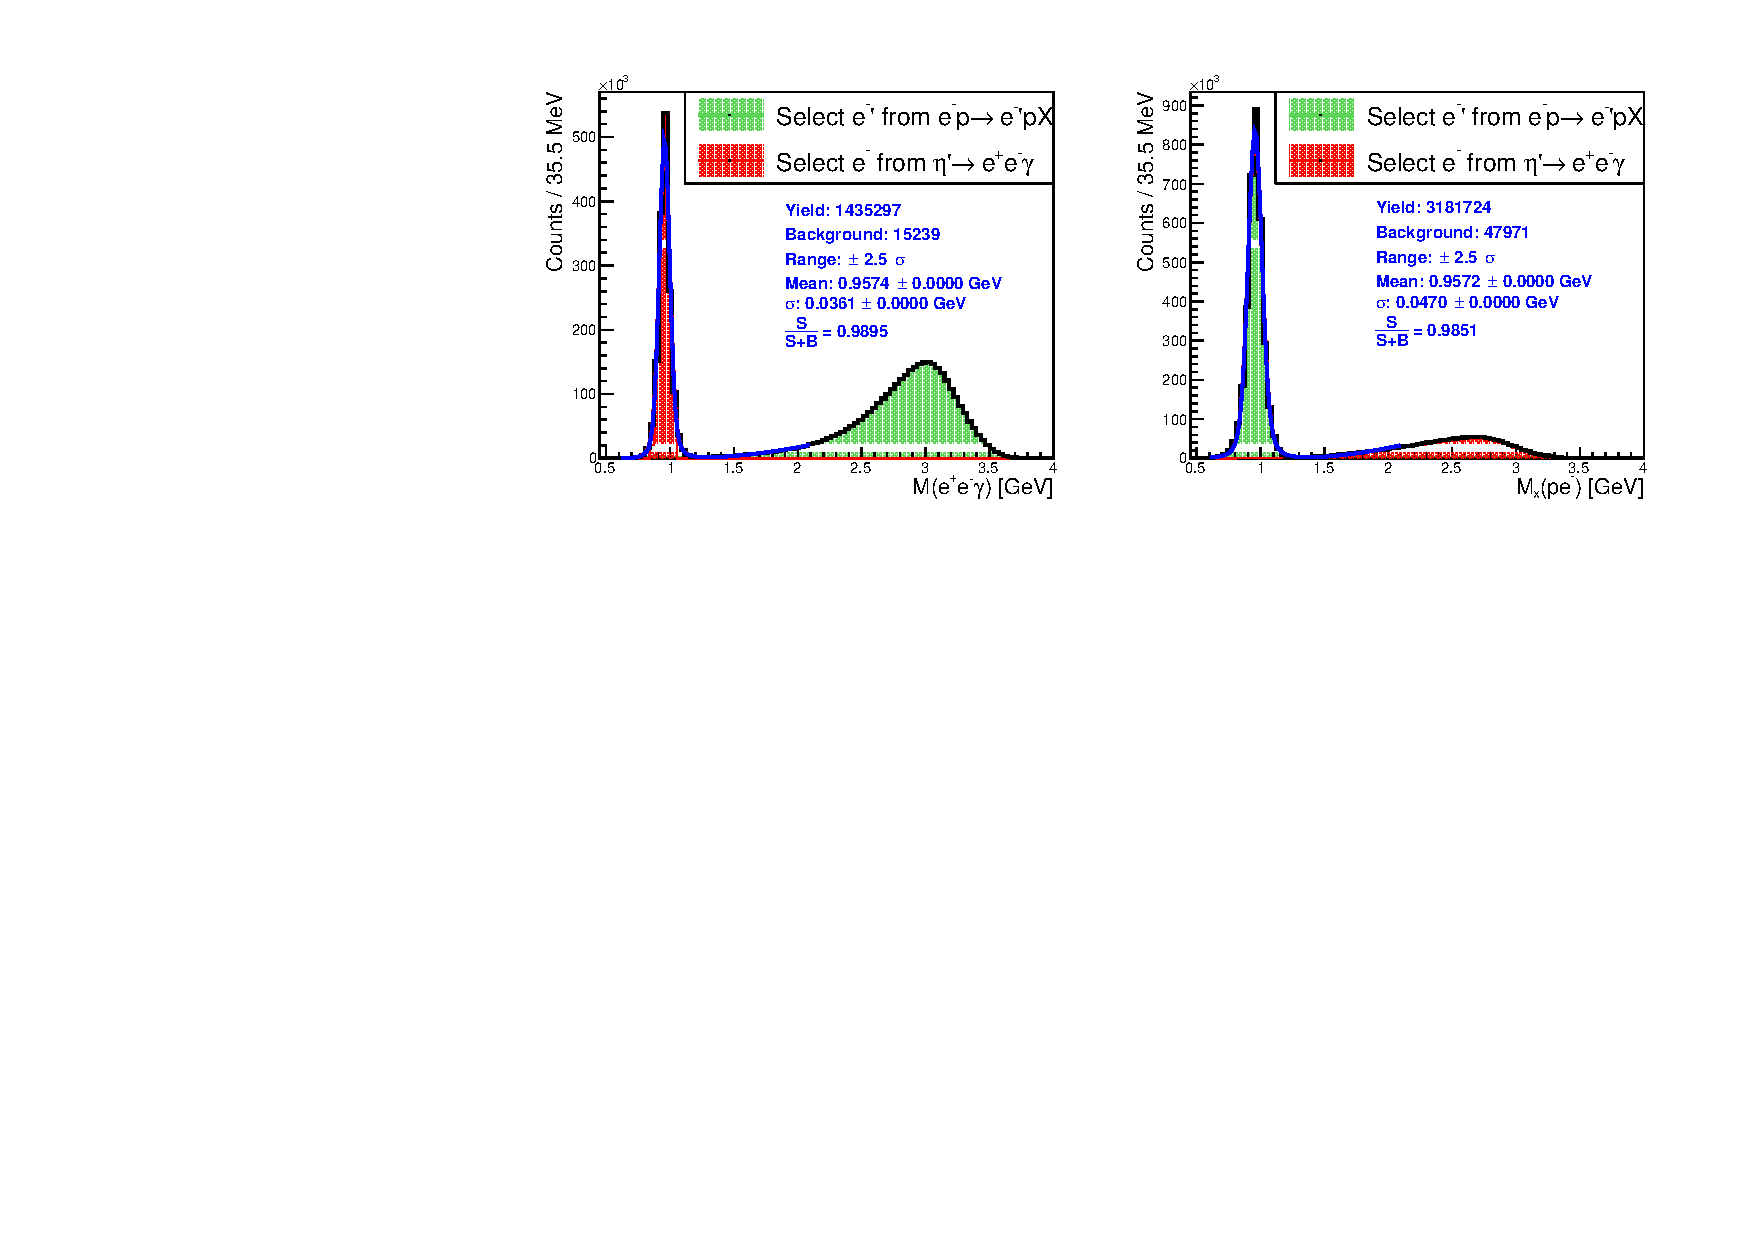
\includegraphics[width=1.2\figwidth,height=1.2\qfigheight]{\grpath/counts/etaPDalitz_contamI.pdf}
		\caption[Reconstrcution with FASTMC]{\label{fig:recon}{(Left) Invariant mass of $\epem \gamma$. (Right) Missing mass off of the proton and one $e^-$.  Red corresponds to the Dalitz $e^-$ being detected and selected, while green is when the scattered beam $e^-$ is detected and rejected. Blue line is a fit using a Voigtian + $2^{\mathrm{nd}}$ order polynomial.}}
	\end{center}\end{figure}
	\FloatBarrier
After placing a cut of $2.5\sigma$ from the mean value of the fit for the left diagram in Fig.~\ref{fig:recon}, we conclude from Fig.~\ref{fig:recondalitz} that the background from leakage of the incorrect $e^-$ is negligible.
\begin{figure}[h!]\begin{center}
		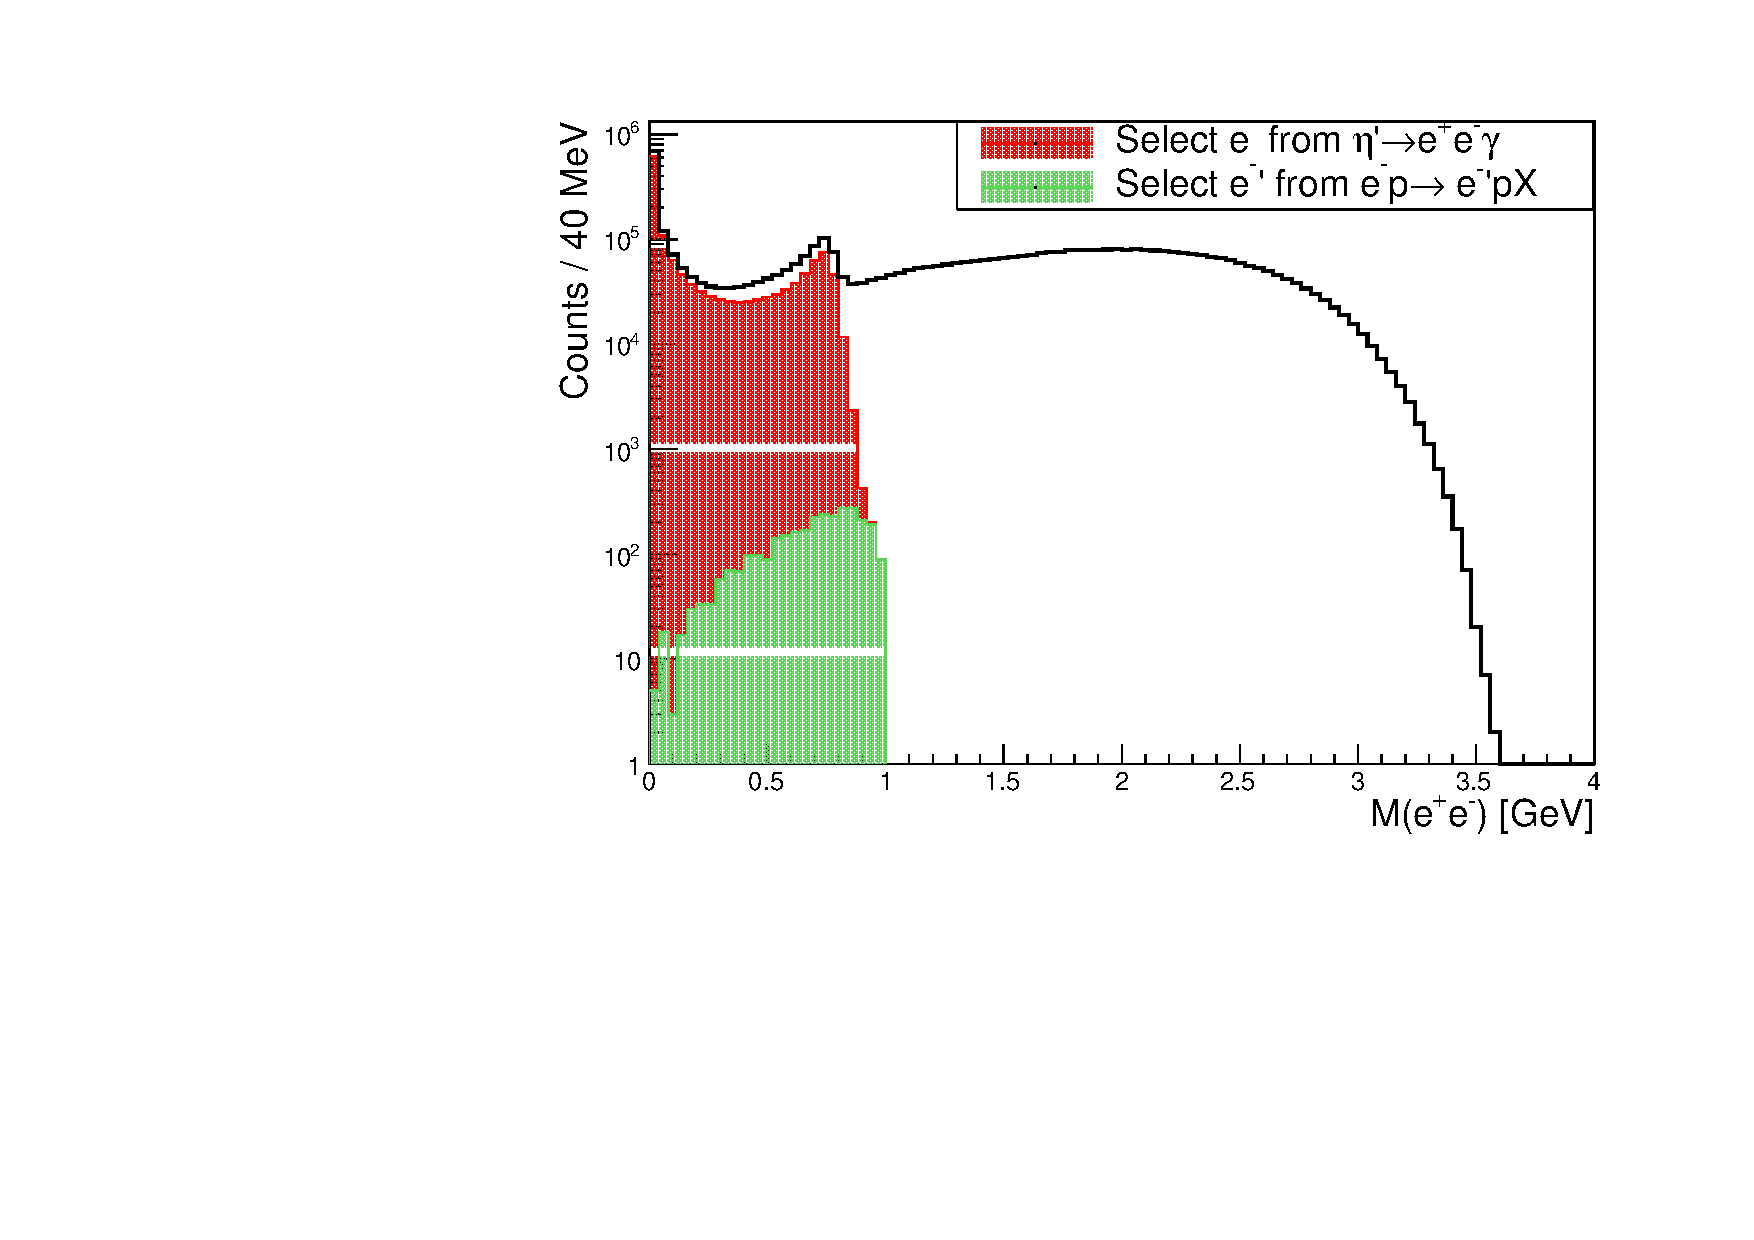
\includegraphics[width=\figwidth,height=1.2\qfigheight]{\grpath/counts/etaPDalitz_contamII.pdf}
		\caption[Reconstrcution with FASTMC]{\label{fig:recondalitz}{Invariant mass of $\epem$.  Red corresponds to the Dalitz $e^-$ being detected and selected, while green is when the scattered beam $e^-$ is detected but accepted in the kinematics.}}
	\end{center}\end{figure}
	\FloatBarrier
The acceptance was calculated by dividing the accepted events by the generated events, per $M(\epem)$ bin. The $\etaP$ Dalitz decay acceptance using the VMD model along with the acceptance using a flat \epemT \ mass distribution can be seen in Fig.\ref{fig:VMDaccepted}.
\begin{figure}[h!]\begin{center}
		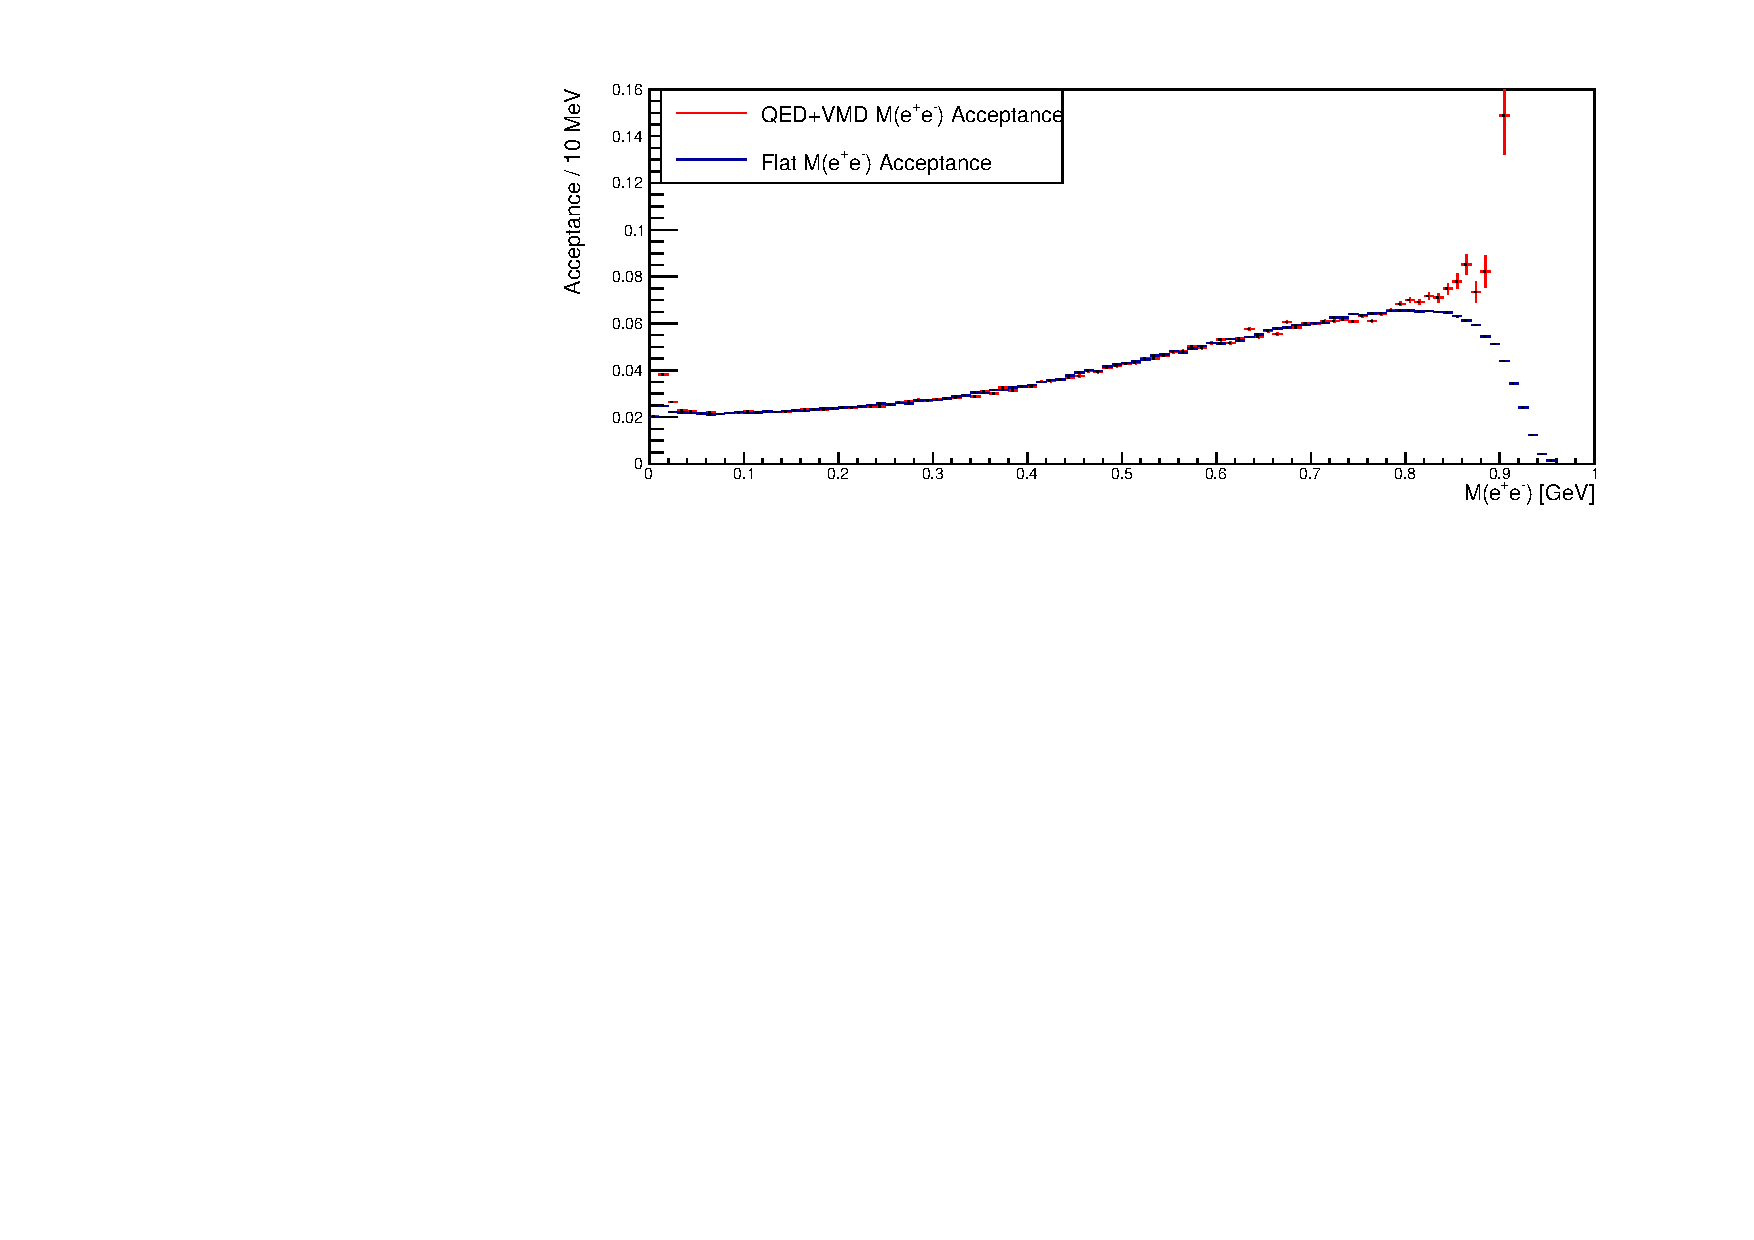
\includegraphics[width=\figwidth,height=1.2\qfigheight]{\grpath/counts/acceptance.pdf}
		\caption[Acceptance as a function of $M(\epem)$]{\label{fig:VMDaccepted}{(Color Online)Acceptance as a function of $M(\epem)$ using two decay models.}}
	\end{center}\end{figure}
\FloatBarrier
\paragraph{Acceptance at 100\% Torus field}
An addition simulation was performed using the same generated data shown above, the difference being the setting of the torus magnetic field. Below, in Fig.~\ref{fig:ratio}, the ratio of the lepton acceptance for the two different torus settings is depicted.
\begin{figure}[h!]\begin{center}
		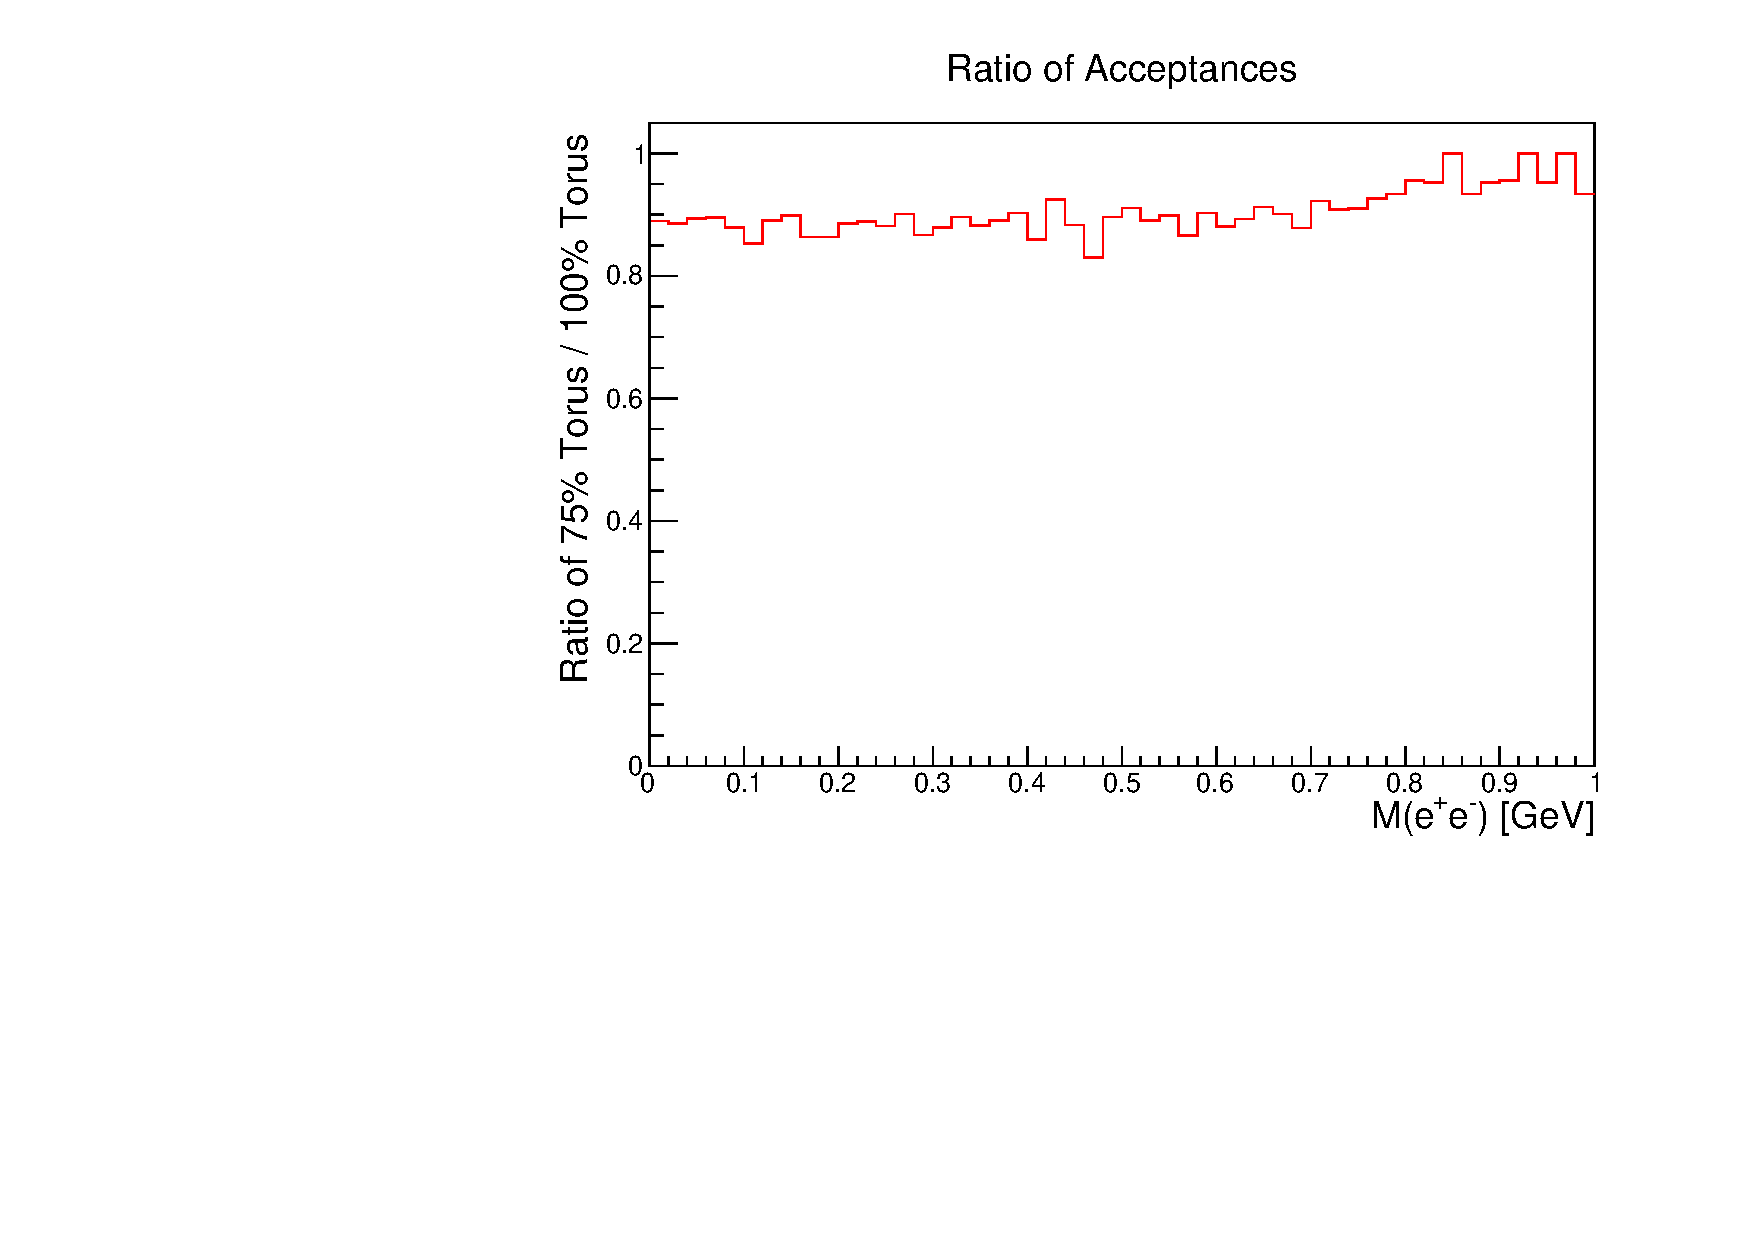
\includegraphics[width=\figwidth,height=1.6\qfigheight]{\grpath/counts/Ratio.pdf}
		\caption[Acceptance, as a function of $M(\epem)$]{\label{fig:ratio}{Ratio of acceptances using a VMD decay model using two torus field settings (75\% and 100\%), as a function of $M(\epem)$. }}
	\end{center}\end{figure}
	\FloatBarrier
\subsection{Calculating the Expected Yield}\label{sec:yield}
%\subsubsection{Calculating Photon Flux}\label{sec:calflux}
%A simple method for calculating the photon flux in CLAS12 is as follows; Using the fact that g12 had a photon flux of $7\cdot 10^7 \ \mathrm{\gamma/s}$ on a Au radiator of $10^{-4} \chi_0$ an expected $\sim 4\cdot 10^9  \mathrm{\gamma/s}$ will be seen in CLAS12 at ${\cal L} = 10^{35}\mathrm{cm^{-2}s^{-1}}$ on a 5~cm $\ell H_2$ target which is $\sim 5.7\cdot 10^{-3} \chi_0$. This number has been independently confirmed in a previous CLAS proposal~\cite{clas.proposal.meson}.

The expected yield for $ep\to e'p \etaP [\etaP\rightarrow p e^+e^- \gamma ]$ is calculated under the assumption, that the $\etaP$ electro-production cross-section can be deduced from the $\etaP$ photo-production cross-section. A qualitative justification of this assumption may be found in Fig.~\ref{fig:EtaProdX}. The shape of the cross-section distributions for $ep\rightarrow e'p\eta$, shown in the top row of Fig.~\ref{fig:EtaProdX}, are comparable to the corresponding distribution for $\gamma p\rightarrow p\eta$, plotted in the bottom row of Fig.~\ref{fig:EtaProdX}. Therefore we use this information as a quasi-realistic model for electro-production of the $\etaP$ meson.
%The major difference is related to the scaling rule of $1/Q^2$, i.e. the electro-production cross-section might be approximated by the photo-production cross-section by scaling down the latter one by $1/Q^2$.

\begin{figure}[htbp]\begin{center}
		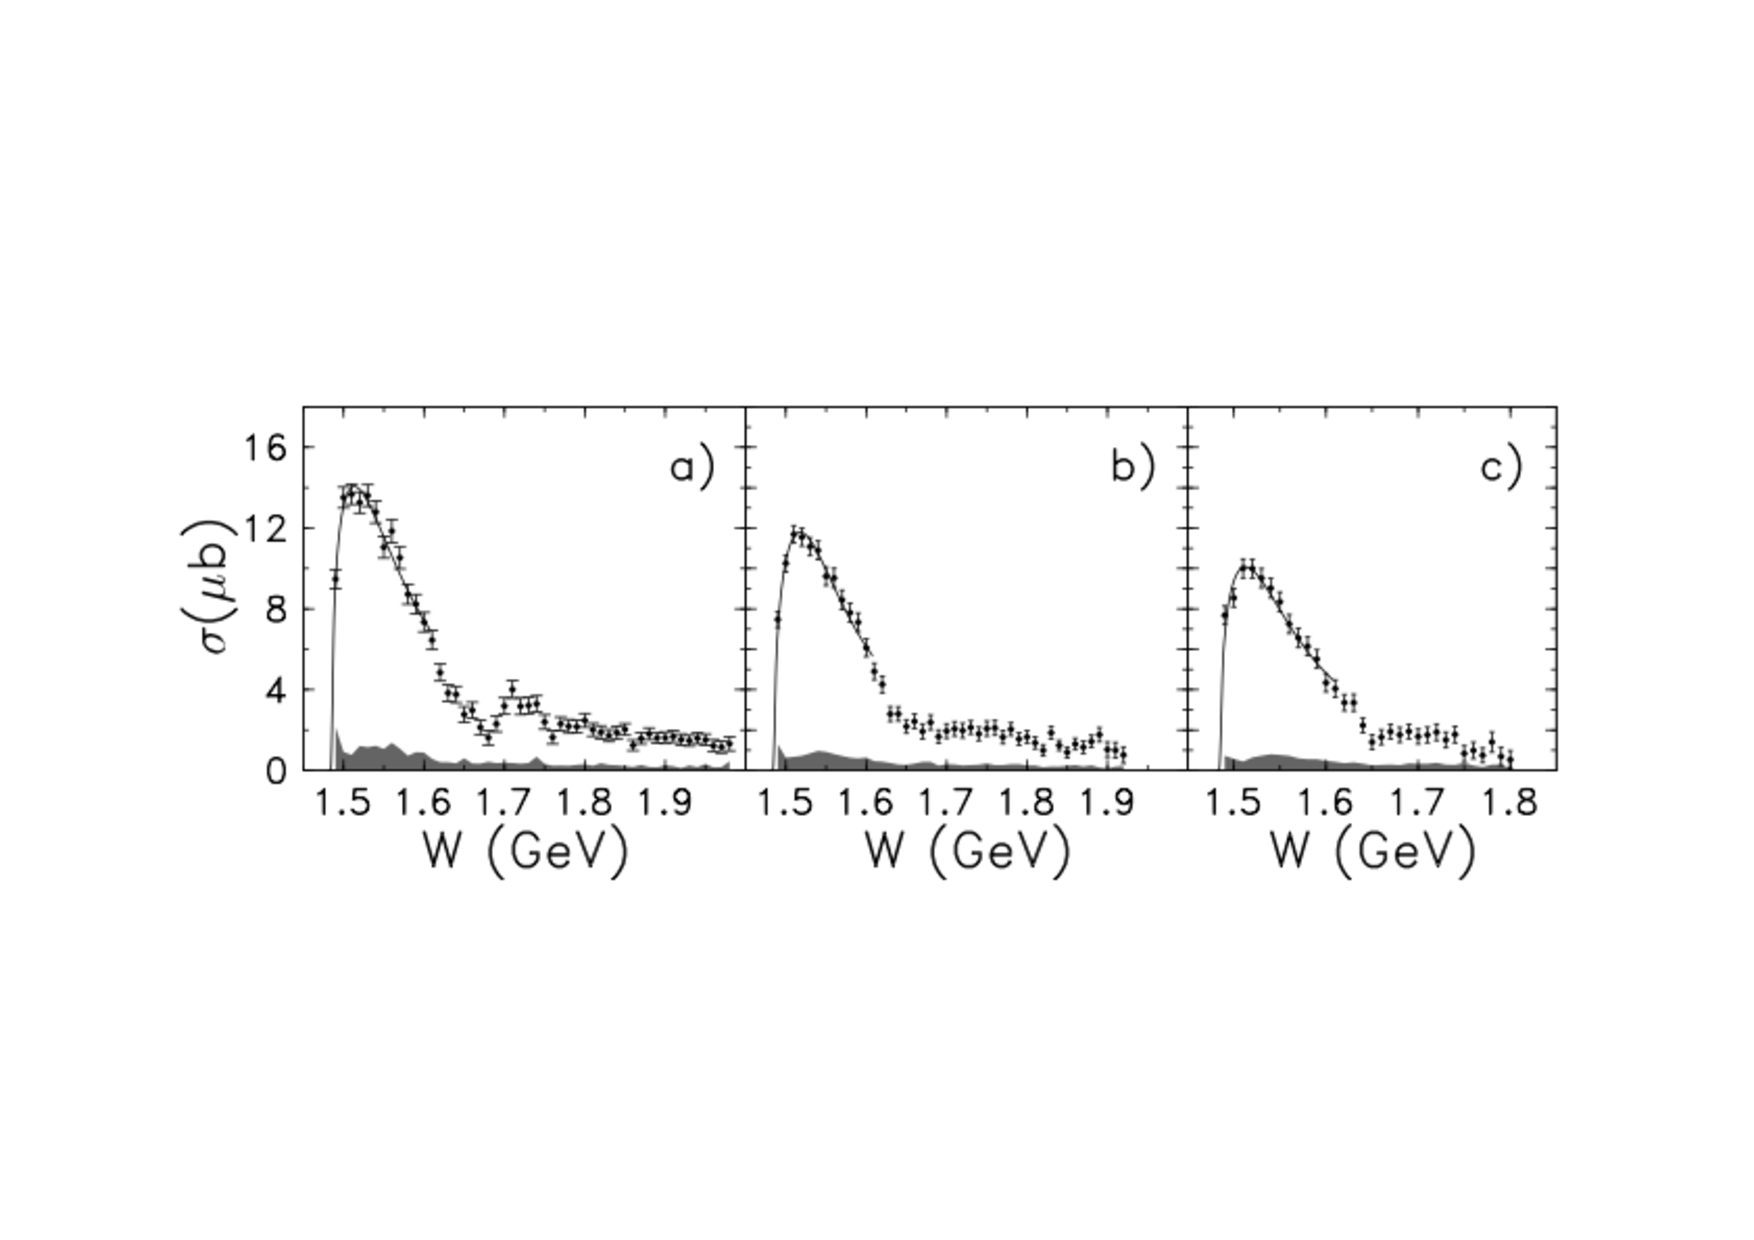
\includegraphics[width=\figwidth,height=1.2\qfigheight]{\grpath/XSection/eta_phot_electXSection.pdf}\\
		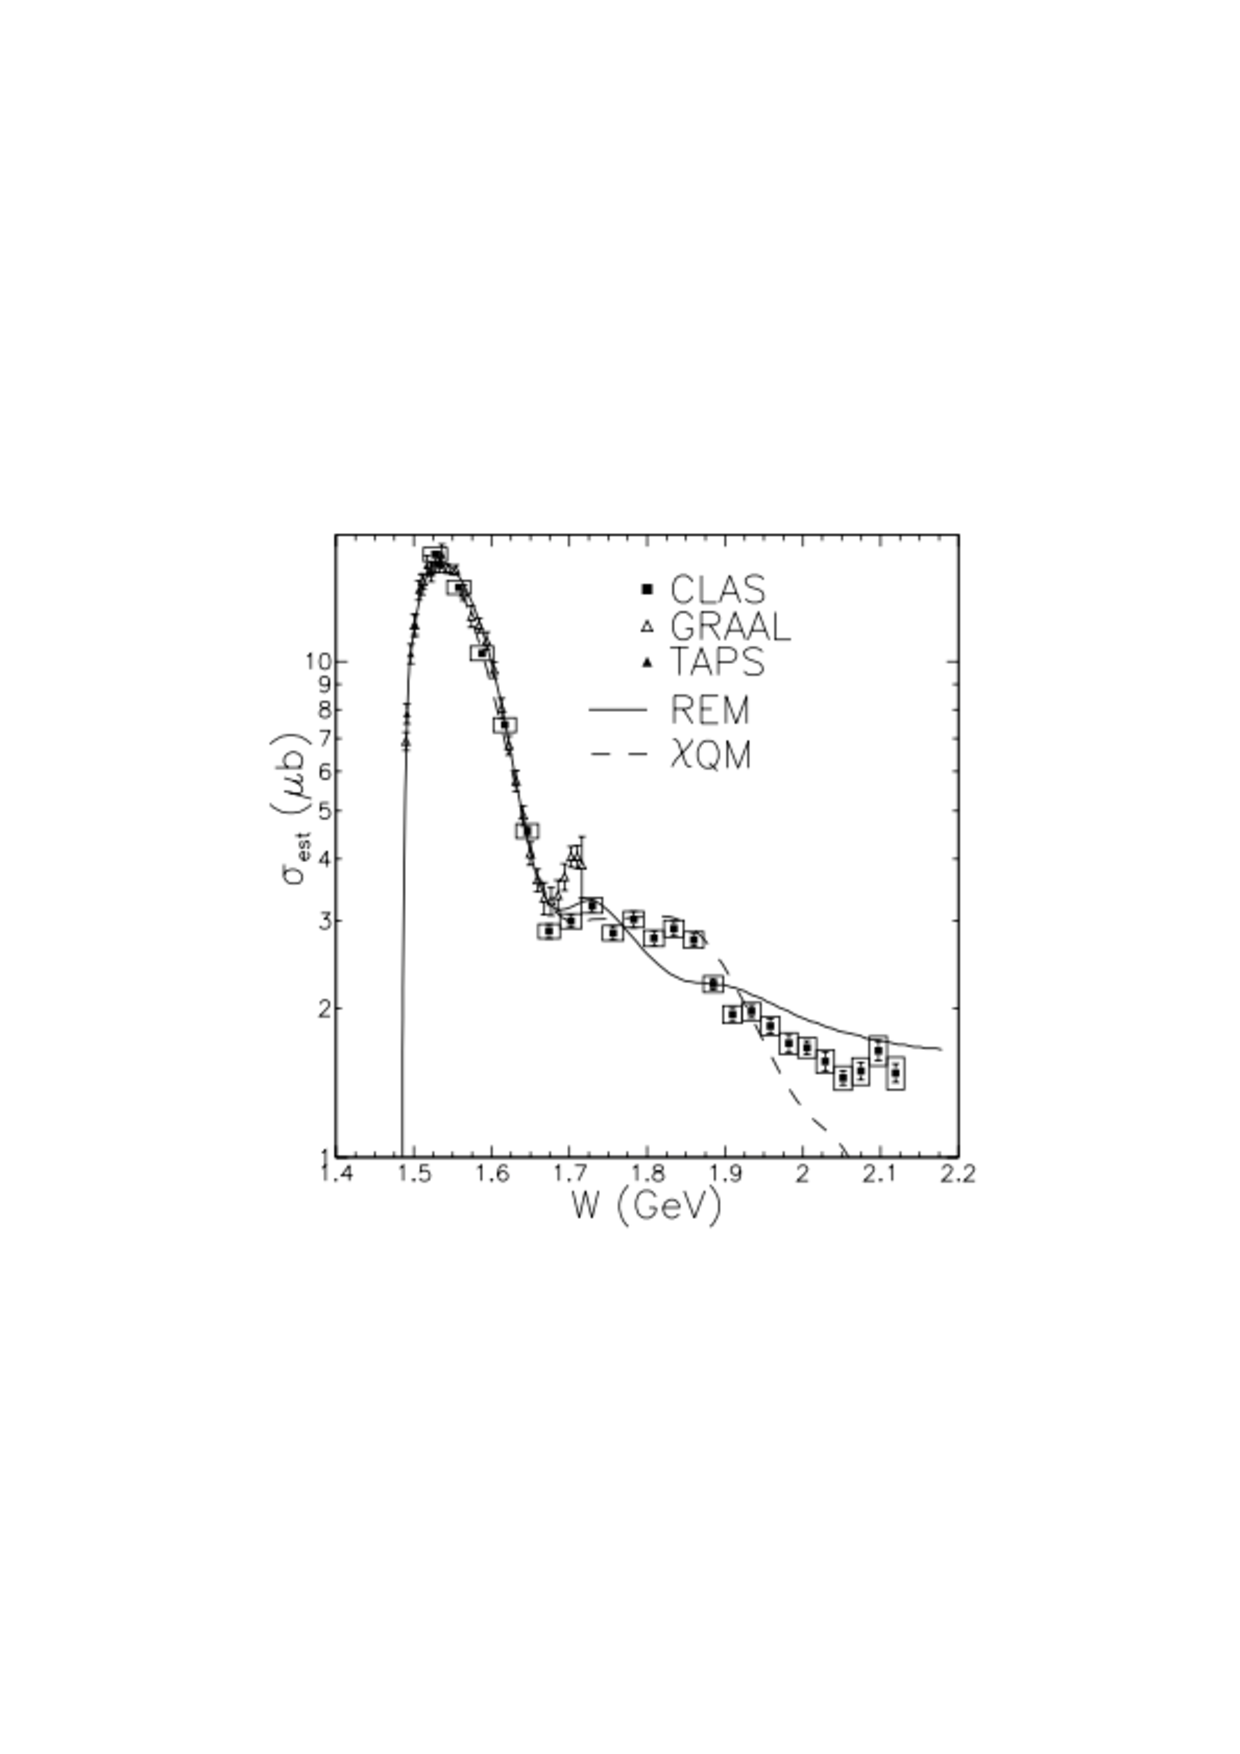
\includegraphics[width=0.7\figwidth,height=0.9\qfigheight]{\grpath/XSection/eta_phot_prodXSection.pdf}
		\caption[eta el-prod. XSection]{\label{fig:EtaProdX}{Integrated cross-section for $ep\to e'p\eta$ (Top) for: (a) $Q^2=0.625(GeV/c)^2$, (b) $Q^2=0.875(GeV/c)^2$, (a) $Q^2=1.125(GeV/c)^2$~\cite{etaelect} and for $\gamma p\rightarrow p\eta$ (Bottom)~\cite{etaphoto}.}}
\end{center}\end{figure}

\FloatBarrier

The top row of Fig.~\ref{fig:EtaPProdX} shows the total photo-production cross-section for hadrons in comparison with the photo-production cross-section for $\etaP$ (see bottom row of Fig.~\ref{fig:EtaPProdX}). Due to the considerations made above, these two cross-section distributions might be directly translated to the corresponding electro-production cross-sections. Using the distributions shown in Fig.~\ref{fig:EtaPProdX}, one might define the following ratio $R(W)$:

\begin{equation}
 R(W) = \frac{\sigma(W)}{\etaP\text{ integrated } \sigma(W)}
\label{XsecR}
\end{equation}

\begin{figure}[h!]\begin{center}
		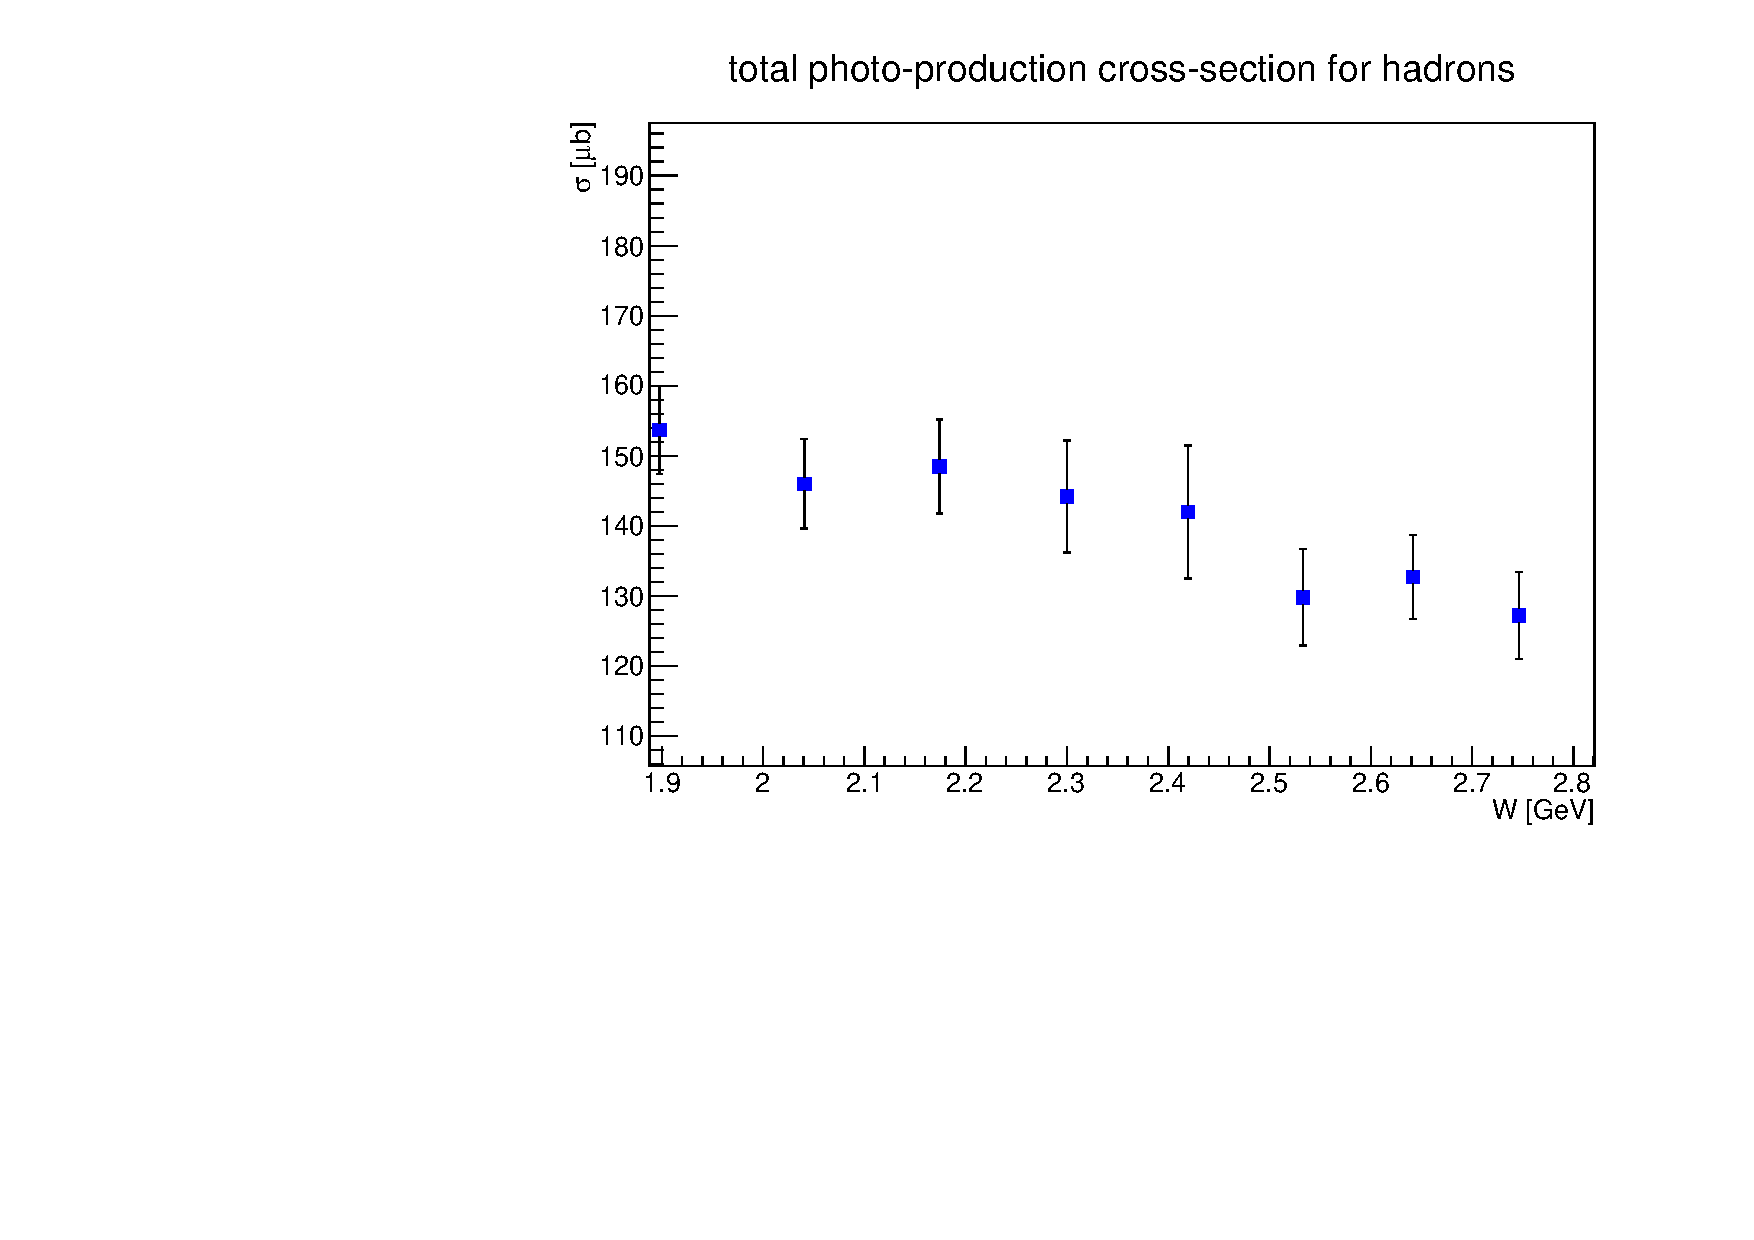
\includegraphics[width=0.9\figwidth,height=0.9\qfigheight]{\grpath/XSection/hadron_prod_photoproduction.pdf}\\
		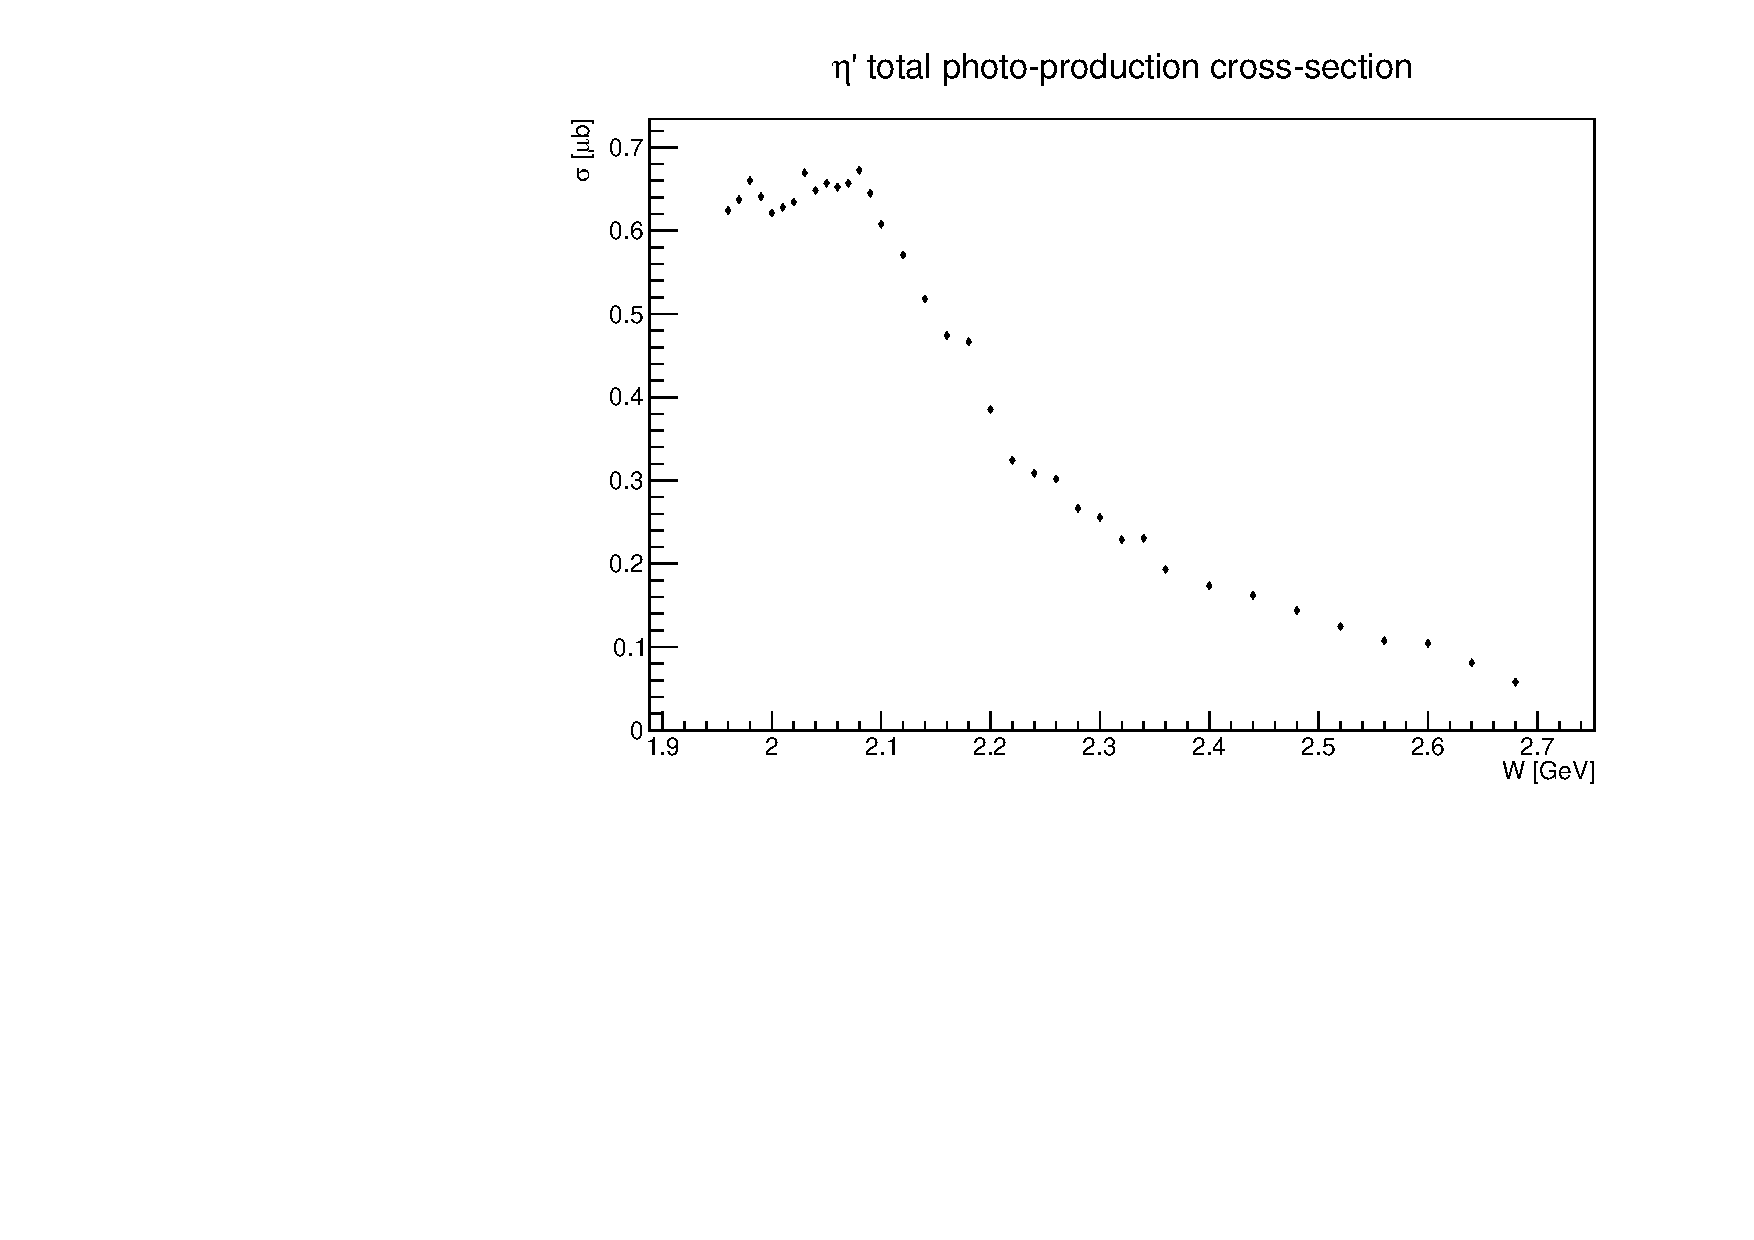
\includegraphics[width=0.9\figwidth,height=0.9\qfigheight]{\grpath/XSection/eta_prod_photoproduction.pdf}
		\caption[etaP phot-prod. XSection]{\label{fig:EtaPProdX}{Integrated cross-section for $\gamma p\rightarrow pX$ (Top) and $\gamma p\rightarrow p\etaP$ (Bottom) as a function of $W$.}}
\end{center}\end{figure}

The rate for mesons in electro-production where the scattered electron is left undetected (W=1.9-2.7~GeV) is $\sim 80\,\rm{kHz}$~\cite{Sargsyan}. This rate needs to be scaled down by $R(W)$ in order to achieve the corresponding rate for $\etaP$ production. This leads to:

\begin{equation}
 \etaP\text{ total rates / 80 Days }(W) = 80\,\rm{kHz}\cdot \frac{86,400\mathrm{\ seconds}}{\text{80 days}}\cdot \frac{1}{R(W)}
\label{etaPRate}
\end{equation}

A plot of Eq.~\ref{etaPRate} is shown in Fig.~\ref{fig:EtaPRate} (left y-axis). The total $\etaP\rightarrow\epem\gamma$ rates per 80 days, and as a function $W$, is calculated by multiplying Eq.\ref{etaPRate} with the product of the average detection efficiency $\epsilon\approx 5\%$ as well as the branching fraction $\mathcal{BR} = 4.69\cdot10^{-4}$~\cite{BESIII} for $\etaP\rightarrow\epem\gamma$. The corresponding plot is shown in Fig.~\ref{fig:EtaPRate} (right y-axis). The total number $N_{tot}$ of expected $\etaP\rightarrow\epem\gamma$ events after 80 days of measurement is given by the integral of Fig.~\ref{fig:EtaPRate} over $W$. This leads to the expected yield:

\begin{equation}
  N_{tot} = \int\limits_{1.9\,\rm{GeV}}^{2.8\,\rm{GeV}} \Big[ {\color{red}{N(W)_{\etaP\rightarrow\epem\gamma\text{ / 80 Days }}}} \Big]dW = \mathrm{\frac{28,200 \ events}{80 Days}}
\label{yield}
\end{equation}


\begin{figure}[h!]\begin{center}
		\includegraphics[width=1.0\figwidth,height=1.4\qfigheight]{\grpath/XSection/Total_rates.pdf}\\
		\caption[etaP rates]{\label{fig:EtaPRate}{Total $\etaP$ production rate per 80 days (left y-axis) and total $\etaP\rightarrow \epem\gamma$ rates per 80 days (right y-axis) as a function of $W$. Both rates have been calculated according to Eq.~\ref{etaPRate}}}
\end{center}\end{figure}

It should be noted that there will be $\etaP$ \ mesons produced from untagged Bremsstrahlung production which should be of the order $\approx 10$~kHz. This would increase the total Dalitz yield by $\approx$3000 events. 

Instead of using an average efficiency $\epsilon \sim 5\%$ for determining the expected yield, one could utilize the $M(\epem)$ dependent acceptance shown in Fig.~\ref{fig:VMDaccepted} to calculate the total expected yield using the same procedure as explained above. This number of events expected to be reconstructed as well as the acceptance corrected yield can be seen in Fig.~\ref{fig:counts} which is consistent with the previous number quoted in Eq.~\ref{yield}.

\begin{figure}[h!]\begin{center}
		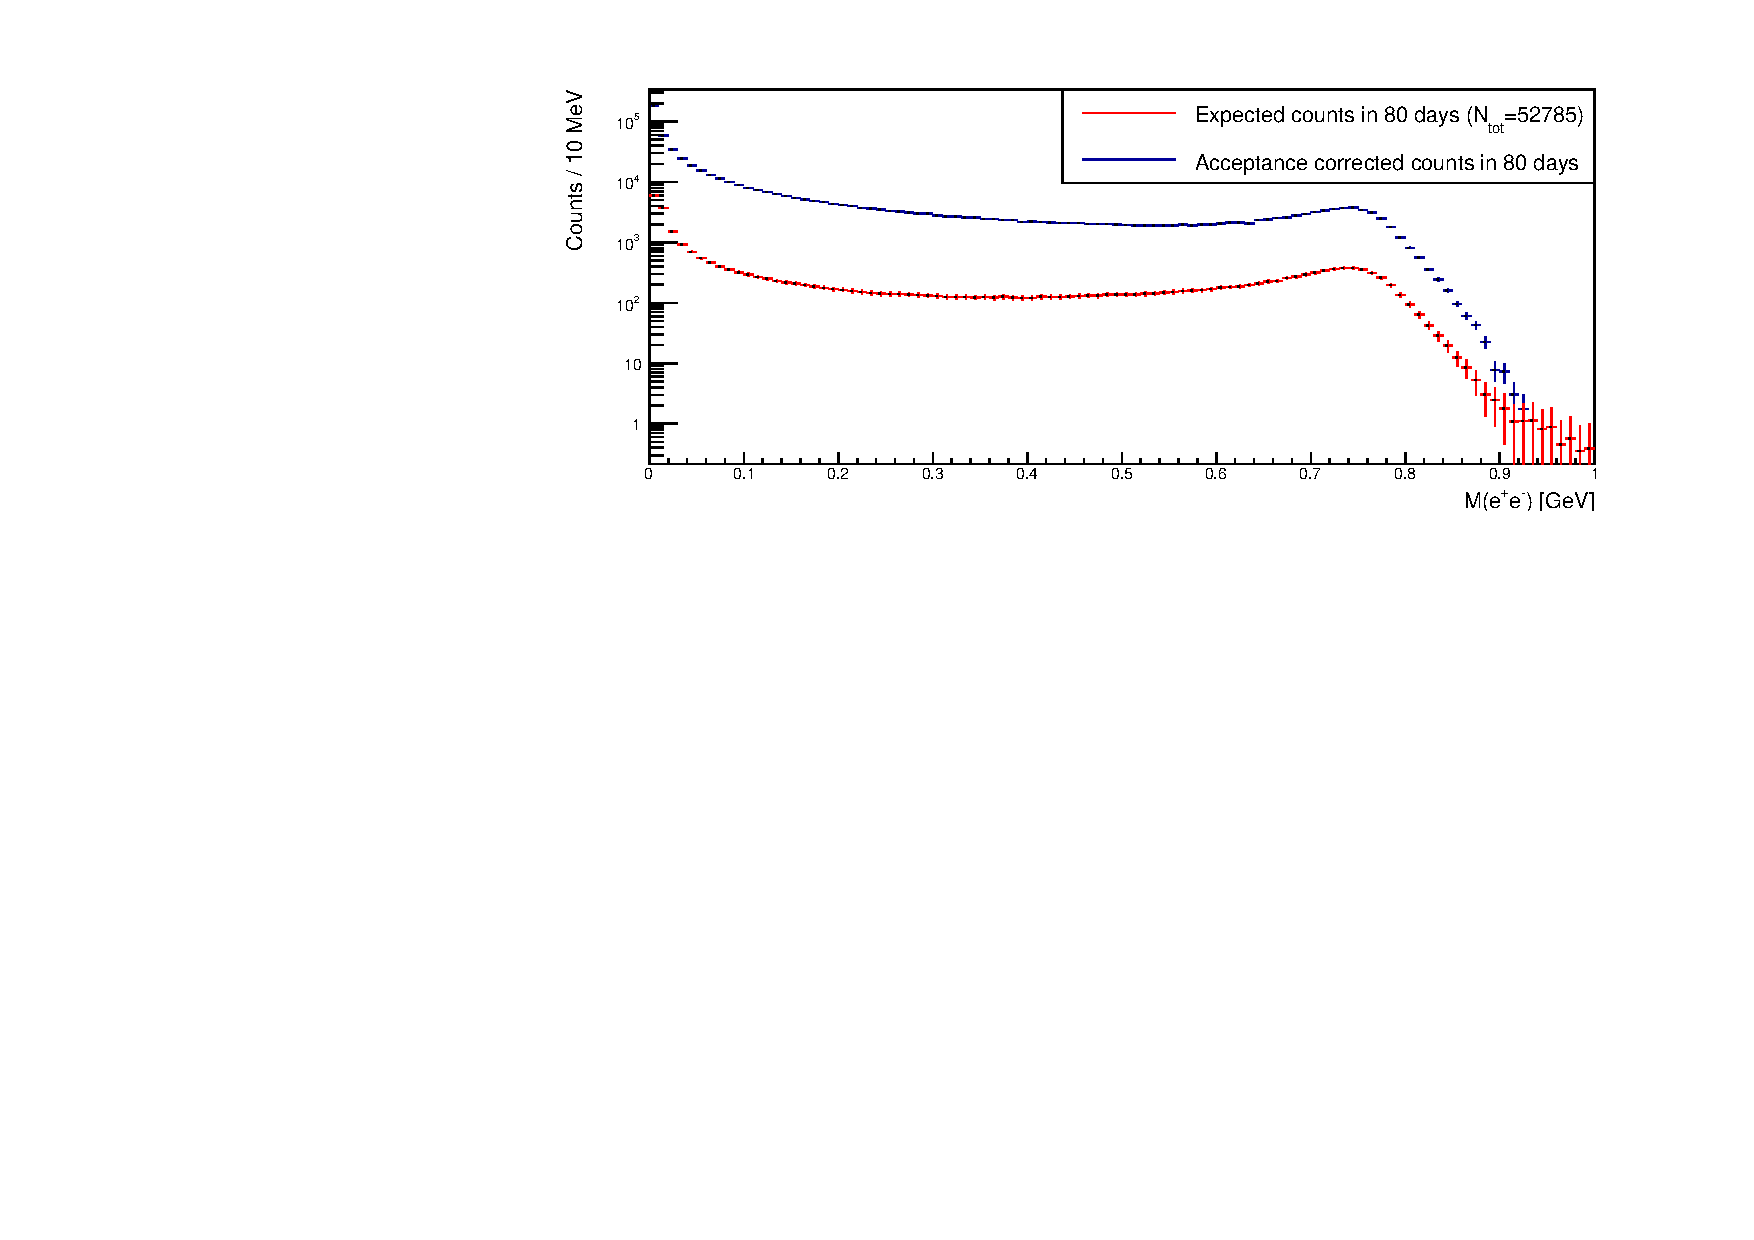
\includegraphics[width=\figwidth,height=1.3\qfigheight]{\grpath/counts/counts.pdf}
		\caption[Acceptance as a function of $M(\epem)$]{\label{fig:counts}{(Color Online)Expected yield as a function of $M(\epem)$.}}
	\end{center}\end{figure}

	\begin{figure}[h!]\begin{center}
			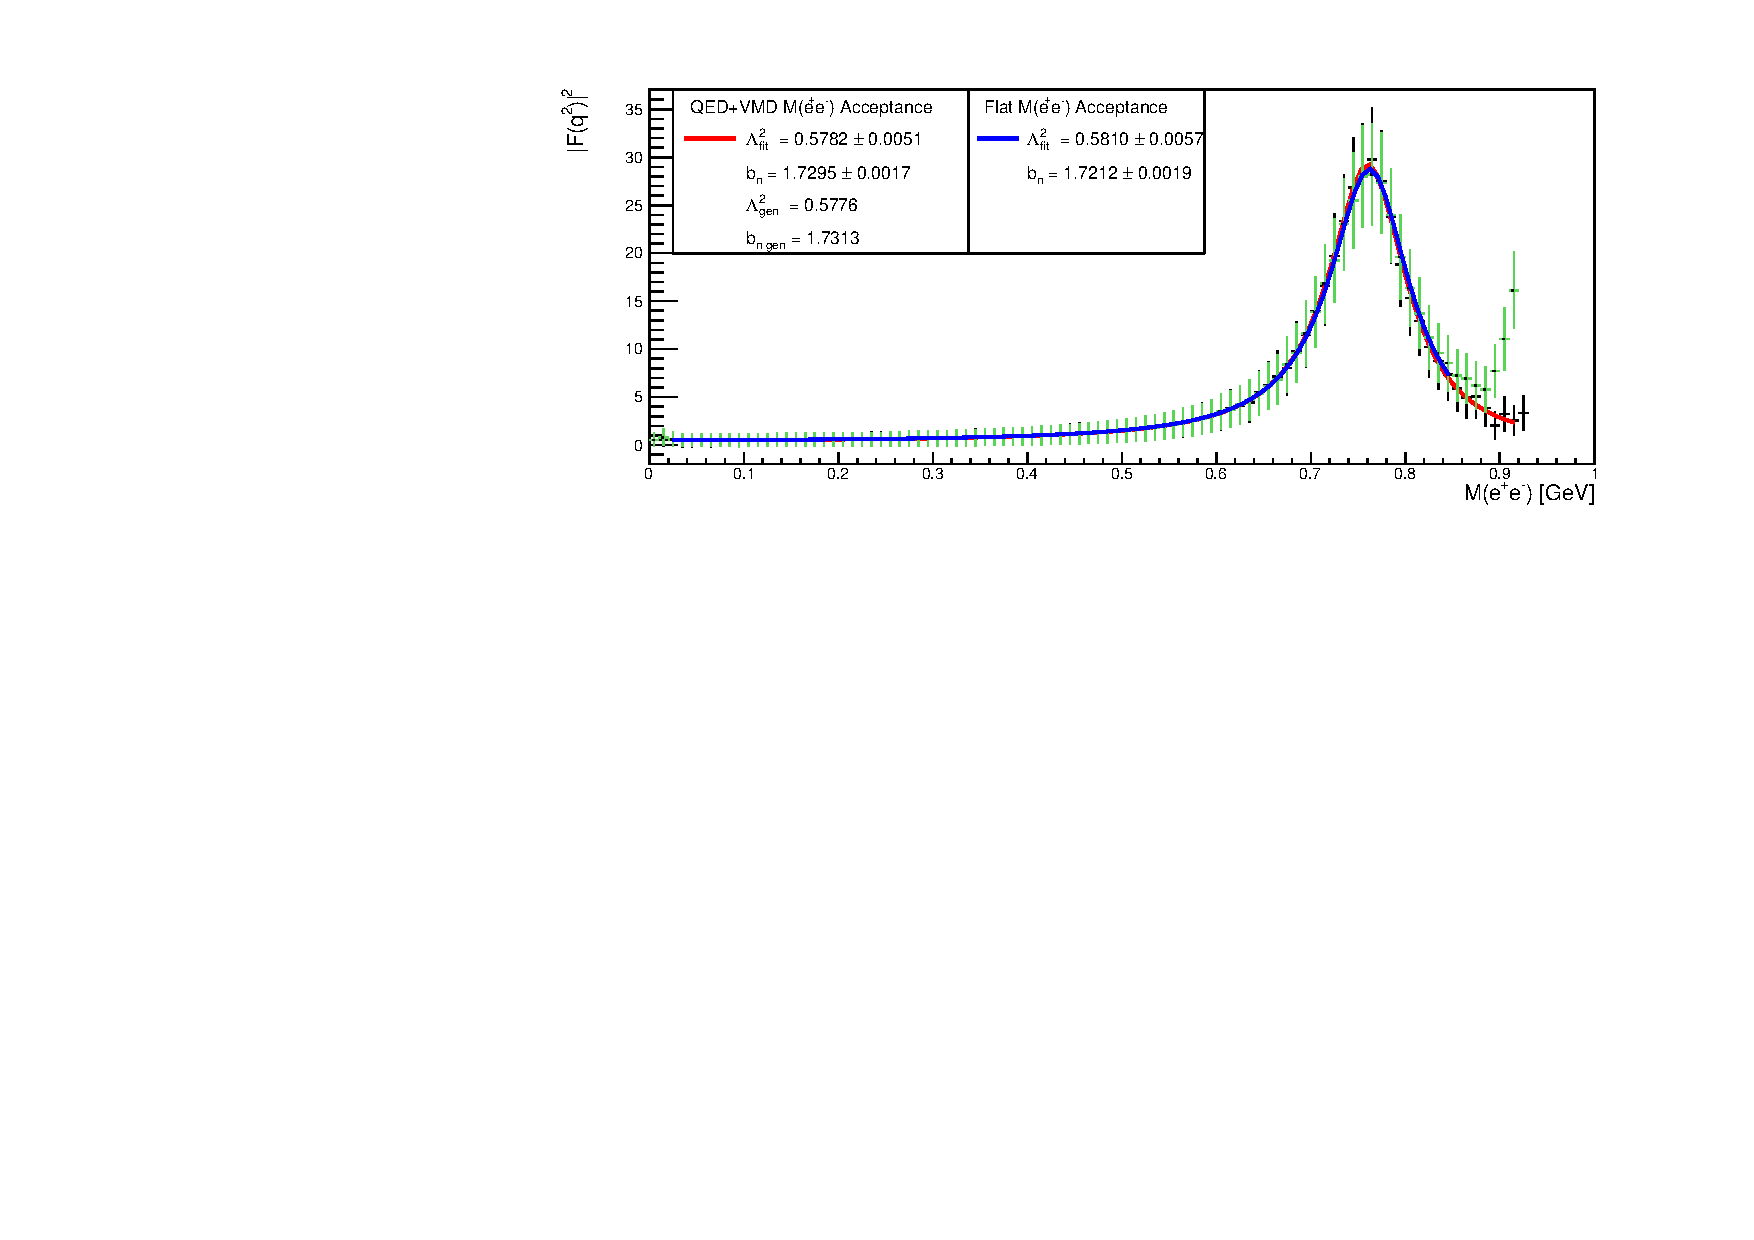
\includegraphics[width=\figwidth,height=1.3\qfigheight]{\grpath/counts/result.pdf}
			\caption[TFF as a function of $M(\epem)$]{\label{fig:results}{(Color Online)$\left|F(q^2)\right|^2$ as a function of $M(\epem)$ using two acceptance models. (black points) QED+VMD $M(\epem)$ acceptance model. (green points) Flat $M(\epem)$ acceptance model. The solid lines represent a fit using Eq.~\ref{TFFbitch} to the data points.}}
		\end{center}\end{figure}

	\FloatBarrier
	From Fig.~\ref{fig:counts} the QED normalized spectrum can be deduced and is shown in Fig.~\ref{fig:results}. Both acceptance models (i.e. flat and QED+VMD) are used to determine the transition form factor. It is shown that there exists a systematic uncertainty depending on the chosen acceptance model. However, the final calculation on the slope parameter or the TFF shows a negligible impact of this uncertainty. Regardless of the acceptance model, it is shown in Fig.~\ref{fig:results} that the accumulated statistics collected by CLAS12 allow for a precision of each parameter $\lesssim 0.5\%$. Compared to current experimental uncertainties of 10\% and differences in theoretical approaches of $\approx$ 10\%~\ref{tab:theory}, this proposed measurement by CLAS12 would not only be in the position to decisively discriminate between the theoretical predictions, but also pin down one of the largest uncertainties to the muon g-2 anomaly.
\subsection{Expected Systematic Uncertainties}
The major sources of systematic uncertainties are the acceptance and particle identification. The di-lepton acceptance uncertainty is estimated to be $\lesssim$ 5\% which was observed in former CLAS experiments. The lepton identification uncertainty will arise from the performance of the HTCC, PCAL and EC. From simulation studies performed for this proposal, all leptons and final state photons are detected within the geometric space of the PCAL+EC with hit coincidences in both. Furthermore, all leptons, within a few percent, that were detected in the PCAL+EC were also detected in the HTCC. Further systematics from pion contamination are mitigated by the pion rejection factor described above. Systematics related to external photon conversion are minimal due to the  1~mm resolution of the primary vertex given by the Silicon Vertex Tracker (SVT) as shown in Sec~\ref{sec:intro.conversion}. Any Bethe-Heitler contributions are negligible when utilizing and exclusive meson reconstruction scheme. To estimate the systematic uncertainty on the expected slope parameter and TFF a 5\% increase in di-lepton acceptance as a function of $M(\epem)$ was applied, i.e.
\begin{align}
\epsilon_{new} = \epsilon \cdot (1+0.05 \cdot M(\epem)) \label{eq:sys} 
\end{align}
As seen in Fig.~\ref{fig:EPEMsys} the systematic arising from the di-lepton uncertainty can be calculated to be:
\begin{align}
b_{n}^{sys} =0.0497 \% \\
\Lambda^{2}_{sys} = 0.0494 \%\ .
\end{align}
\begin{figure}[h!]\begin{center}
		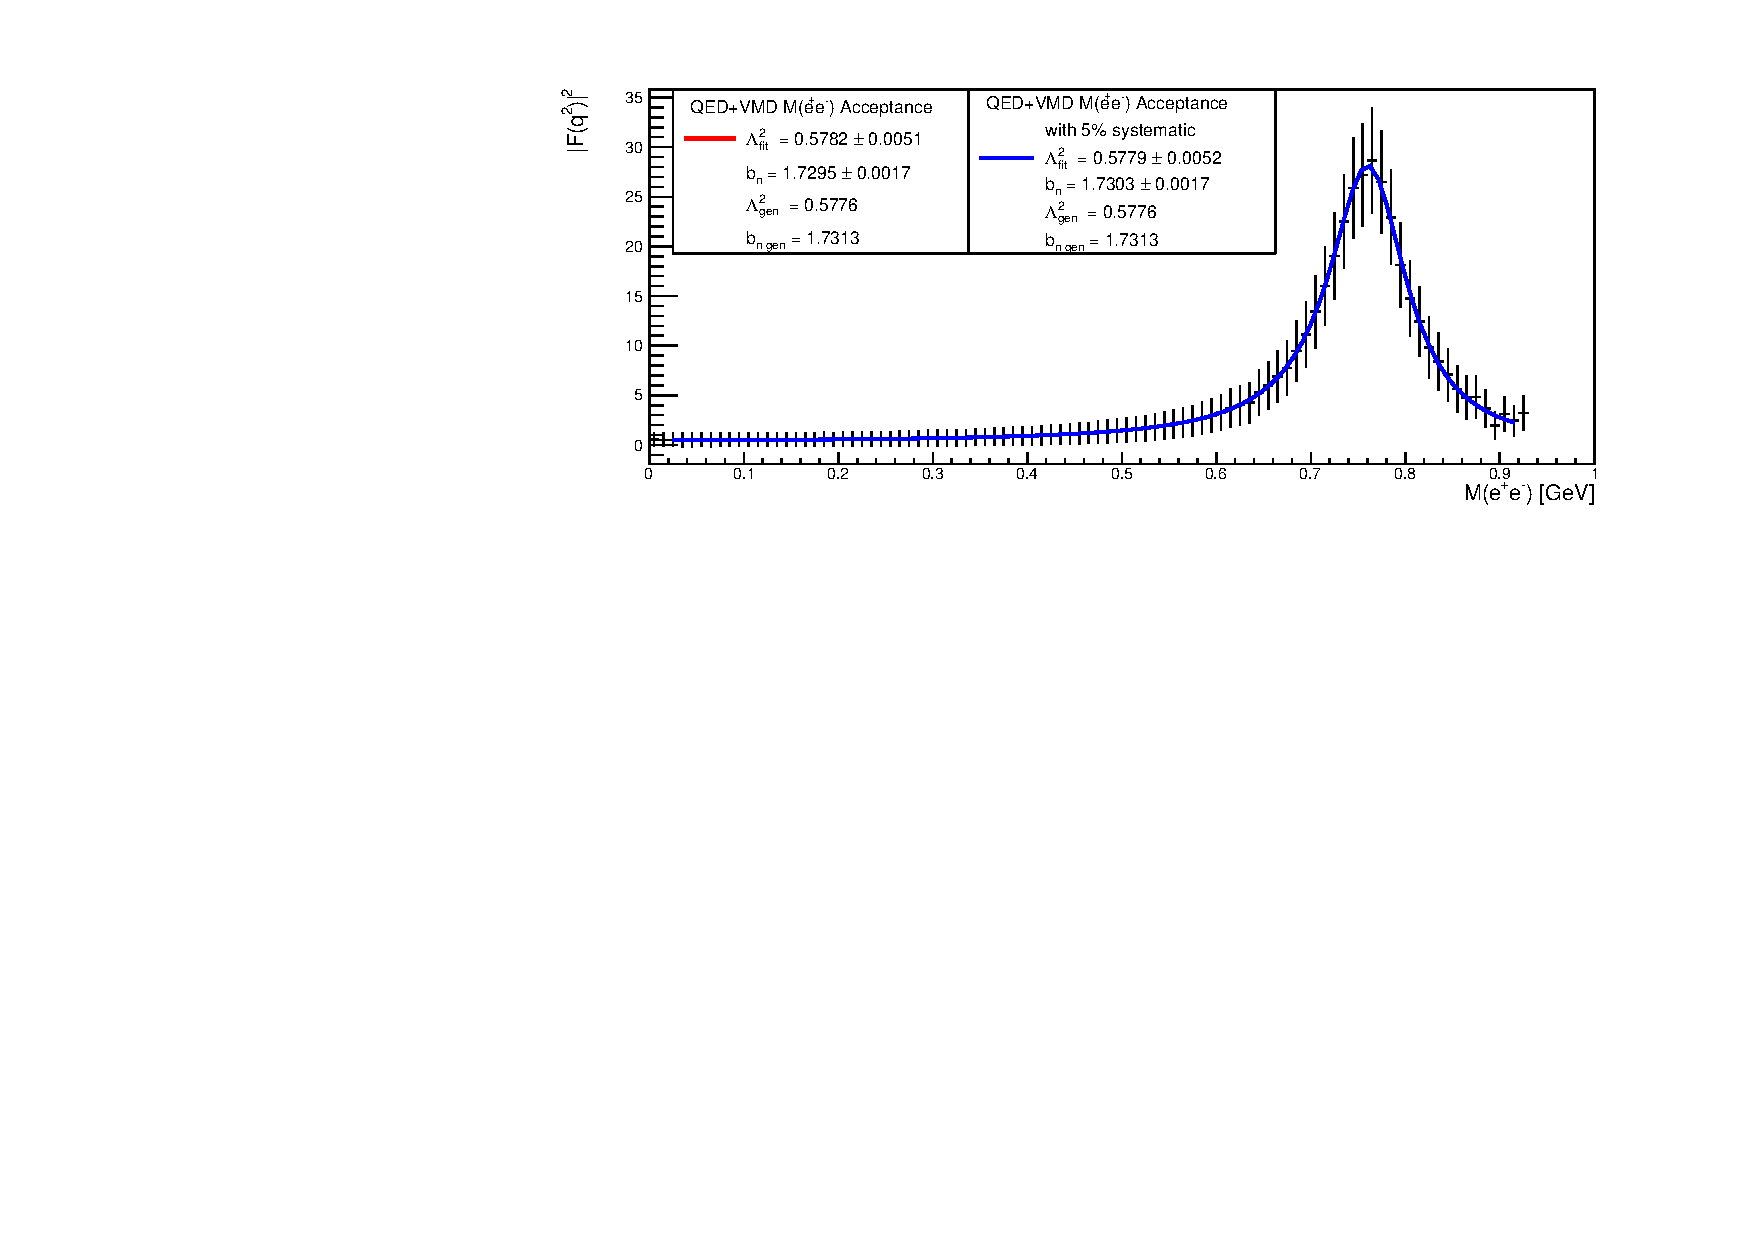
\includegraphics[width=\figwidth,height=1.3\qfigheight]{\grpath/counts/sys.pdf}
		\caption[Acceptance as a function of $M(\epem)$]{\label{fig:EPEMsys}{(Color Online)Expected yield as a function of $M(\epem)$ with a gradual 5\% increase in $M(\epem)$ acceptance .}}
	\end{center}\end{figure}
	\FloatBarrier

